\documentclass[10pt]{article}
\usepackage[T1]{fontenc}

% Document Details
\newcommand{\CLASS}{CSE 521}
\newcommand{\assigmentnum}{Problem Set 3}

\usepackage[margin = 1.5in]{geometry}
\usepackage{titling}
\setlength{\droptitle}{-6em}   % This is your set screw
\date{}
\renewcommand{\maketitle}{
	\clearpage
	\begingroup  
	\centering
	\LARGE \sffamily\textbf{\CLASS} \Large \assigmentnum\\[.8em]
	\large Tyler Chen\\[1em]
	\endgroup
	\thispagestyle{empty}
}
 % Title Styling


\usepackage{enumitem}

% Figures
\usepackage{subcaption}

% TikZ and Graphics
\usepackage{tikz, pgfplots}
\pgfplotsset{compat=1.12}
\usetikzlibrary{patterns,arrows}
\usepgfplotslibrary{fillbetween}

\usepackage{pdfpages}
\usepackage{adjustbox}

\usepackage{lscape}
\usepackage{titling}
\usepackage[]{hyperref}


% Header Styling
\usepackage{fancyhdr}
\pagestyle{fancy}
\lhead{\sffamily \CLASS}
\rhead{\sffamily Chen \textbf{\thepage}}
\cfoot{}

% Paragraph Styling
\setlength{\columnsep}{1cm}
\setlength{\parindent}{0pt}
\setlength{\parskip}{5pt}
\renewcommand{\baselinestretch}{1}

% TOC Styling
\usepackage{tocloft}
\iffalse
\renewcommand{\cftsecleader}{\cftdotfill{\cftdotsep}}

\renewcommand\cftchapafterpnum{\vskip6pt}
\renewcommand\cftsecafterpnum{\vskip10pt}
\renewcommand\cftsubsecafterpnum{\vskip6pt}

% Adjust sectional unit title fonts in ToC
\renewcommand{\cftchapfont}{\sffamily}
\renewcommand{\cftsecfont}{\bfseries\sffamily}
\renewcommand{\cftsecnumwidth}{2em}
\renewcommand{\cftsubsecfont}{\sffamily}
\renewcommand{\cfttoctitlefont}{\hfill\bfseries\sffamily\MakeUppercase}
\renewcommand{\cftaftertoctitle}{\hfill}

\renewcommand{\cftchappagefont}{\sffamily}
\renewcommand{\cftsecpagefont}{\bfseries\sffamily}
\renewcommand{\cftsubsecpagefont}{\sffamily}
\fi
 % General Styling
% Code Display Setup
\usepackage{listings,lstautogobble}
\usepackage{lipsum}
\usepackage{courier}
\usepackage{catchfilebetweentags}

\lstset{
	basicstyle=\small\ttfamily,
	breaklines=true, 
	frame = single,
	rangeprefix=,
	rangesuffix=,
	includerangemarker=false,
	autogobble = true
}


\usepackage{algorithmicx}
\usepackage{algpseudocode}

\newcommand{\To}{\textbf{to}~}
\newcommand{\DownTo}{\textbf{downto}~}
\renewcommand{\algorithmicdo}{\hspace{-.2em}\textbf{:}}
 % Code Display Setup
% AMS MATH Styling
\usepackage{amsmath, amssymb}
\newcommand{\qed}{\hfill\(\square\)}

%\newtheorem*{lemma}{Lemma} 
%\newtheorem*{theorem}{Theorem}
%\newtheorem*{definition}{Definition}
%\newtheorem*{prop}{Proposition}
%\renewenvironment{proof}{{\bfseries Proof.}}{}


% mathcal
\newcommand{\cA}{\ensuremath{\mathcal{A}}}
\newcommand{\cB}{\ensuremath{\mathcal{B}}}
\newcommand{\cC}{\ensuremath{\mathcal{C}}}
\newcommand{\cD}{\ensuremath{\mathcal{D}}}
\newcommand{\cE}{\ensuremath{\mathcal{E}}}
\newcommand{\cF}{\ensuremath{\mathcal{F}}}
\newcommand{\cG}{\ensuremath{\mathcal{G}}}
\newcommand{\cH}{\ensuremath{\mathcal{H}}}
\newcommand{\cI}{\ensuremath{\mathcal{I}}}
\newcommand{\cJ}{\ensuremath{\mathcal{J}}}
\newcommand{\cK}{\ensuremath{\mathcal{K}}}
\newcommand{\cL}{\ensuremath{\mathcal{L}}}
\newcommand{\cM}{\ensuremath{\mathcal{M}}}
\newcommand{\cN}{\ensuremath{\mathcal{N}}}
\newcommand{\cO}{\ensuremath{\mathcal{O}}}
\newcommand{\cP}{\ensuremath{\mathcal{P}}}
\newcommand{\cQ}{\ensuremath{\mathcal{Q}}}
\newcommand{\cR}{\ensuremath{\mathcal{R}}}
\newcommand{\cS}{\ensuremath{\mathcal{S}}}
\newcommand{\cT}{\ensuremath{\mathcal{T}}}
\newcommand{\cU}{\ensuremath{\mathcal{U}}}
\newcommand{\cV}{\ensuremath{\mathcal{V}}}
\newcommand{\cW}{\ensuremath{\mathcal{W}}}
\newcommand{\cX}{\ensuremath{\mathcal{X}}}
\newcommand{\cY}{\ensuremath{\mathcal{Y}}}
\newcommand{\cZ}{\ensuremath{\mathcal{Z}}}

% mathbb
\usepackage{bbm}
\newcommand{\bOne}{\ensuremath{\mathbbm{1}}}

\newcommand{\bA}{\ensuremath{\mathbb{A}}}
\newcommand{\bB}{\ensuremath{\mathbb{B}}}
\newcommand{\bC}{\ensuremath{\mathbb{C}}}
\newcommand{\bD}{\ensuremath{\mathbb{D}}}
\newcommand{\bE}{\ensuremath{\mathbb{E}}}
\newcommand{\bF}{\ensuremath{\mathbb{F}}}
\newcommand{\bG}{\ensuremath{\mathbb{G}}}
\newcommand{\bH}{\ensuremath{\mathbb{H}}}
\newcommand{\bI}{\ensuremath{\mathbb{I}}}
\newcommand{\bJ}{\ensuremath{\mathbb{J}}}
\newcommand{\bK}{\ensuremath{\mathbb{K}}}
\newcommand{\bL}{\ensuremath{\mathbb{L}}}
\newcommand{\bM}{\ensuremath{\mathbb{M}}}
\newcommand{\bN}{\ensuremath{\mathbb{N}}}
\newcommand{\bO}{\ensuremath{\mathbb{O}}}
\newcommand{\bP}{\ensuremath{\mathbb{P}}}
\newcommand{\bQ}{\ensuremath{\mathbb{Q}}}
\newcommand{\bR}{\ensuremath{\mathbb{R}}}
\newcommand{\bS}{\ensuremath{\mathbb{S}}}
\newcommand{\bT}{\ensuremath{\mathbb{T}}}
\newcommand{\bU}{\ensuremath{\mathbb{U}}}
\newcommand{\bV}{\ensuremath{\mathbb{V}}}
\newcommand{\bW}{\ensuremath{\mathbb{W}}}
\newcommand{\bX}{\ensuremath{\mathbb{X}}}
\newcommand{\bY}{\ensuremath{\mathbb{Y}}}
\newcommand{\bZ}{\ensuremath{\mathbb{Z}}}

% alternative mathbb
\newcommand{\NN}{\ensuremath{\mathbb{N}}}
\newcommand{\RR}{\ensuremath{\mathbb{R}}}
\newcommand{\CC}{\ensuremath{\mathbb{C}}}
\newcommand{\ZZ}{\ensuremath{\mathbb{Z}}}
\newcommand{\EE}{\ensuremath{\mathbb{E}}}
\newcommand{\PP}{\ensuremath{\mathbb{P}}}
\newcommand{\VV}{\ensuremath{\mathbb{V}}}
\newcommand{\cov}{\ensuremath{\text{Co}\VV}}
% Math Commands

\newcommand{\st}{~\big|~}
\newcommand{\stt}{\text{ st. }}
\newcommand{\ift}{\text{ if }}
\newcommand{\thent}{\text{ then }}
\newcommand{\owt}{\text{ otherwise }}

\newcommand{\norm}[1]{\left\lVert#1\right\rVert}
\newcommand{\snorm}[1]{\lVert#1\rVert}
\newcommand{\ip}[1]{\ensuremath{\left\langle #1 \right\rangle}}
\newcommand{\pp}[3][]{\frac{\partial^{#1}#2}{\partial #3^{#1}}}
\newcommand{\dd}[3][]{\frac{\d^{#1}#2}{\d #3^{#1}}}
\renewcommand{\d}{\ensuremath{\mathrm{d}}}

\newcommand{\indep}{\rotatebox[origin=c]{90}{$\models$}}




 % Math shortcuts
\usepackage{mdframed}

\newenvironment{algorithm}[1][\@nil]
{\def\tmp{#1}%
\begin{mdframed}[
  frametitle={Algorithm. \ifx\tmp\@nnil  \else \normalfont (#1) \fi},
  linecolor=green!70,
  linewidth=1,
  topline=false,
  bottomline=false,
  rightline=false,
  rightmargin=.5cm
]}
{\end{mdframed}}

\newenvironment{method}[1][\@nil]
{
\def\tmp{#1}%
\begin{mdframed}[
  frametitle={Method. \ifx\tmp\@nnil  \else \normalfont (#1) \fi},
  linecolor=violet!70,
  linewidth=1,
  topline=false,
  bottomline=false,
  rightline=false,
  rightmargin=.5cm
]}
{\end{mdframed}}

\newenvironment{definition}[1][\@nil]
{\def\tmp{#1}%
\begin{mdframed}[
  frametitle={Definition. \ifx\tmp\@nnil  \else \normalfont (#1) \fi},
  linecolor=blue!70,
  linewidth=1,
  topline=false,
  bottomline=false,
  rightline=false,
  rightmargin=.5cm
]}
{\end{mdframed}}

\newenvironment{theorem}[1][\@nil]
{\def\tmp{#1}%
\begin{mdframed}[
  frametitle={Theorem. \ifx\tmp\@nnil  \else \normalfont (#1) \fi},
  linecolor=red!70,
  linewidth=1,
  topline=false,
  bottomline=false,
  rightline=false,
  rightmargin=.5cm
]}
{\end{mdframed}}

\newenvironment{lemma}[1][\@nil]
{\def\tmp{#1}%
\begin{mdframed}[
  frametitle={Lemma. \ifx\tmp\@nnil  \else \normalfont (#1) \fi},
  linecolor=red!70,
  linewidth=1,
  topline=false,
  bottomline=false,
  rightline=false,
  rightmargin=.5cm
]}
{\end{mdframed}}

\newenvironment{proof}[1][\@nil]
{\def\tmp{#1}%
\begin{mdframed}[
  frametitle={Proof. \ifx\tmp\@nnil  \else \normalfont (#1) \fi},
  linecolor=red!30,
  linewidth=1,
  topline=false,
  bottomline=false,
  rightline=false,
  rightmargin=.5cm
]}
{\end{mdframed}}



 % Proof shortcuts
% Problem
\usepackage{floatrow}

\newenvironment{problem}[1][]
{\pagebreak
\noindent\rule{\textwidth}{1pt}\vspace{0.25em}
{\sffamily \textbf{#1}}
\par
}
{\par\vspace{-0.5em}\noindent\rule{\textwidth}{1pt}}

\newenvironment{solution}[1][]
{{\sffamily \textbf{#1}}
\par
}
{}

 % Problem Environment

\rhead{\sffamily Tyler Chen \textbf{\thepage}}

\newcommand{\tr}{\operatorname{tr}}

\usepackage{placeins}


\begin{document}
\maketitle

\begin{problem}[Problem 1]
Prove the following matrix equations:
\begin{enumerate}[label=(\alph*),nolistsep]
    \item Let \( A\in\RR^{n\times n} \) and let \( U \in \RR^{n\times k} \) be a matrix with orthonormal columns \( U_1,\ldots, U_k \). So, \( UU^T = \sum_{i=1}^{k} U_iU_i^T \) is a projection matrix. Show that,
        \begin{align*}
            \norm{A-UU^TA}_F^2 = \norm{A}_F^2-\norm{U^TA}_F^2
        \end{align*}
        
    \item Let \( A \in \RR^{m\times n} \) and \( B\in\RR^{n\times m} \) show that \( AB \) and \( BA \) have the same nonzero eigenvalues, i.e., if \( ABv = \lambda v \), then there exists a vector \( y \) such that \( BAy = \lambda y \). 

\end{enumerate}
\end{problem}


\begin{solution}[Solution]
\begin{enumerate}[label=(\alph*)]
    \item Recall that for any matrices \( X,Y \), \( \norm{X}_F^2 = \tr(X^T X) \) and that \( \tr(X+Y) = \tr(X) + \tr(Y) \). Note further than \( U^TU = I_k \), the \( k\times k \) identity. Therefore,
        \begin{align*}
            \norm{A-UU^TA}_F^2 &= \tr\left( (A-UU^TA)^T(A-UU^TA) \right)
            \\&= \tr\left( (A^T-A^TUU^T)(A-UU^TA) \right)
            \\&= \tr\left( A^TA -A^TUU^TA-A^TUU^TA + A^TUU^TUU^TA \right)
            \\&= \tr\left( A^TA - A^TUU^TA \right)
            \\&= \tr\left( A^TA \right) - \tr \left(A^TUU^TA \right)
            \\&= \norm{A}_F^2 - \norm{U^TA}_F^2
        \end{align*}
        


    \item Suppose \( AB v = \lambda v \) for some \( \lambda \neq 0 \) and \( v \). Then,
        \begin{align*}
            BA(Bv) = \lambda (Bv)
        \end{align*}

        This proves that \( \lambda \) is an eigenvalue of \( BA \) (with eigenvector \( Bv \)). 
        The reverse direction is proved by relabling \( A \), \( B \), \( m \), \( n \).

        Note that if \( \lambda = 0 \) then we cannot guarantee that \( Bv \neq 0 \) so \( \lambda = 0\) may not be an eigenvalue of \( BA \). 

\end{enumerate}
\end{solution}

\begin{problem}[Problem 2]
    For a vector \( u\in\RR^n \), write \( u\otimes u \) to denote the vector in \( \RR^{n^2} \) where for any \( 1\leq i,j\leq n \), \( (u\otimes u)_{(i-1)n+j} = u_i u_j \).
\begin{enumerate}[label=(\alph*),nolistsep]
    \item Show that for any pair of vectors \( u,v\in\RR^n \), 
        \begin{align*}
            \ip{u\otimes u,v\otimes v} = \ip{u,v}^2
        \end{align*}
        
    \item Let \( A \in \RR^{n\times n} \) be a PSD matrix, and let \( B \in \RR^{n\times n} \) be the matrix where \( B_{i,j} = (A_{i,j})^2 \) Prove that B is PSD.
    \item \textbf{Extra Credit}: Let \( P = \{p_1,\ldots,p_n\} \subset \RR^d \) be a set of points of norm 1. For \( \sigma > 0 \), let \( G_\sigma\in \RR^{n\times n} \) be the Gaussian kernel on \( P \). I.e.,
        \begin{align*}
            G_\sigma(i,j) = \frac{1}{\sqrt{2\pi \sigma}} e^{-\norm{p_i-p_j}^2/2\sigma}
        \end{align*}
    Show that \( G_\sigma \succeq 0 \). 
\end{enumerate}
\end{problem}


\begin{solution}[Solution]
\begin{enumerate}[label=(\alph*)]
    \item 
        We prove a more general result where \( (u\otimes v)_{(i-1)n+j} = u_iv_j \). 

        By definition of inner product, and using the bijection \( k \leftrightarrow (i-1)n+j \) between \( \{1,\ldots,n^2\} \) and \( \{1,\ldots,n\}^2 \),
        \begin{align*}
            \ip{ u\otimes v,x\otimes y} 
            &= \sum_{k=1}^{n^2} (u\otimes v)_k (x\otimes y)_k 
            = \sum_{i=1}^{n} \sum_{i=1}^{n} (u\otimes v)_{(i-1)n+j} (x\otimes y)_{(i-1)n+j} 
        \end{align*}
        Now, applying the definition of \( u \otimes v \) and \( x\otimes y \),
        \begin{align*}
            \ip{u\otimes v,x\otimes y} &= \sum_{i=1}^{n} \sum_{i=1}^{n} u_iv_j x_iy_j
            = \left( \sum_{i=1}^{n} u_ix_i \right) \left( \sum_{j=1}^{n} v_jy_j \right)
            = \ip{u,x}\ip{v,y}
        \end{align*}


    \item 
        We prove the more general result that for two PSD matrices \( C \) and \( D \) that the matrix \( B \) defined by \( B_{i,j} = C_{i,j}D_{i,j} \) is also PSD.

        Since \( C \) and \( D \) are PSD we can write,
        \begin{align*}
            C = UU^T, && D = VV^T
        \end{align*}
        
        Then, denoting the \( i \)-th row of \( U \) by \( U_i \) and the \( i \)-th row of \( V \) by \( V_i \),
        \begin{align*}
            C_{i,j} = \ip{U_i,U_j}, 
            &&
            D_{i,j} = \ip{D_i,D_j}
        \end{align*}

        Therefore,
        \begin{align*}
            D_{i,j} = C_{i,j}D_{i,j} = \ip{U_i,U_j}\ip{V_i,V_j}
            = \ip{ U_i\otimes V_i,U_j\otimes V_j}
        \end{align*}

        But this means \( B = XX^T \) where the \( (i-1)n+j \)-th row of \( X \) is \( U_i\otimes V_j \). Therefore \( B \) is PSD. 

   \item
        Note that \( \norm{p_i-p_j}^2 = \norm{p_i}^2 + \norm{p_j}^2 - \ip{p_i,p_j} = 2-2\ip{p_i,p_j} \). Therefore,
        \begin{align*}
            G_\sigma(i,j) = \frac{1}{\sqrt{2\pi\sigma}}e^{-\norm{p_i-p_j}^2/2\sigma}
            = \frac{e^{-1/\sigma}}{\sqrt{2\pi\sigma}}e^{\ip{p_i,p_j}/\sigma}
        \end{align*}
        
        We then have,
        \begin{align*}
            G_\sigma(i,j) = \frac{e^{-1/\sigma}}{\sqrt{2\pi\sigma}}\sum_{k=1}^{\infty} \frac{\ip{p_i,p_j}^k}{k!} 
        \end{align*}
        
        
        Let \( C_{i,j} = \ip{p_i,p_j} \) and define \( P = [p_1,\ldots,p_t] \) to be the matrix with rows \( p_i \). Then,
        \begin{align*}
            C_{i,j} = \ip{p_i,p_j} = ( P^TP )_{i,j}  
        \end{align*}

        We have show that the matrix with entries \( C_{i,j}^k \) is also PSD. Moreover, the scalar multiple of a PSD matrix is PSD, as is the sum of PSD matrices. Therefore each partial sum is PSD, and since the total sum converges, it is also PSD.
      
      This proves \( G_\sigma \) is PSD.
      

       

\end{enumerate}
\end{solution}


\begin{problem}[Problem 3]
    Let \( A \in R^{n\times n} \). Normally, we need to scan all non-zero entries of \( A \) to compute \( \norm{A}_F^2 \). In this problem,
    we see that if \( A \) is PSD then we can approximate \( \norm{A}_F^2 \) in time \( \cO(n \log(1/\delta)/2) \) with probability at least \( 1 - \delta \). Note that this is sublinear in the number of non-zero entries of \( A \). So, indeed our algorithm does not read all non-zero entries of \( A \).

\begin{enumerate}[label=(\alph*),nolistsep]
    \item First, assume that all diagonal entries of \( A \) are 1, i.e., \( A_{i,i} = 1 \) for all \( i \). Show that for all \( i \neq j\), \( A_{i,j} \leq 1 \).

    \item Still, assume all diagonal entries of \( A \) are 1. Show that by uniformly sampling \( \cO(n/\epsilon^2) \) off-diagonal entries of \( A \), we can approximate \( \norm{A}_F^2 \) with a constant probability.

    \item Now, we solve the general case: In this case, we sample \( A_{i,j} \) with probability \( p_{i,j} = (A_{i,i}A_{j,j})/(\sum_{k,l} A_{k,k}A_{l,l}) \) and if \( i \), \( j \) is sampled we let \( X = (A_{i,j})^2/p_{i,j} \). Show that \( X \) gives an unbiased estimator of \( \norm{A}_F^2 \). Design an algorithm that by sampling \( \cO(n \log(1/\delta)/\epsilon^2 ) \) coordinates of \( A \)) gives a multiplicative \( 1 \pm \epsilon \)  approximation of \( \norm{A}_F^2 \) with probability at least \( 1 - \delta\).
\end{enumerate}
\end{problem}

\begin{solution}[Solution]

Recall the theorem from lecture 5:
    Let \( X_1,\ldots, X_k \) be iid with mean \( \mu \) and relative variance \( t \). Then the average \( (X_1+ \cdots + X_k)/k \) is a \( 1\pm \epsilon \) approximation to \( \mu \) with probability 9/10 for some \( k = \cO(t/\epsilon^2) \).

    Recall that by returning the median of \( \log(1/\delta) \) of such trials the probability of success is boosted to \( 1-\delta \). That is, a \( 1 \pm \epsilon \) multiplicative approximation to \( \mu \) can be obtained with probability \( 1-\delta \) using \( \cO(t\log(1/\delta)/\epsilon^2) \) samples.

\begin{enumerate}[label=(\alph*)]
    \item Assume \( A \) is symmetric positive-semidefinite. Then, \( x^TAx\geq 0 \) for all \( x \). In particular,
        \begin{align*}
            0 &\leq (e_i-e_j)^TA(e_i-e_j) 
            %= e_i^TAe_i + e_i^TAe_j + e_j^TAe_i + e_j^TAe_j
            = A_{i,i} - A_{i,j} - A_{j,i} + A_{j,j}
            = 2 - 2A_{i,j}
        \end{align*}
        
        Therefore \( A_{i,j} \leq A_{i,i} = 1 \).

        Note also that,
        \begin{align*}
            0 \leq (e_i+e_j)^TA(e_i+e_j)
            = A_{i,i} + A_{i,j} + A_{j,i} + A_{j,j}
        \end{align*}
        
        Therefore \( A_{i,j} \geq - A_{i,i} \).

    \item

%        \( n\sum A_{ij}^4 \leq \left( \sum_{}^{} A_{i,j}^2 \right)^2 \)

        Let \( X = n^2 (A_{i,j})^2 \) with probability \( 1/n^2 \). Then,
        \begin{align*}
            \EE[X] = \sum_{i=1}^{n} \sum_{j=1}^{n} \PP[\text{choose }i,j] \: n^2 (A_{i,j})^2 
            = \sum_{i=1}^{n} \sum_{j=1}^{n} (A_{i,j})^2
            = \norm{A}_F^2
        \end{align*}
        
        Similarly,
        \begin{align*}
            \EE[X^2] = \sum_{i=1}^{n} \sum_{j=1}^{n} \PP[\text{choose }i,j] \: (n^2 A_{i,j}^2)^2 
            = \sum_{i=1}^{n} \sum_{j=1}^{n} n^2(A_{i,j})^4
        \end{align*}

        When the diagonal entries of \( A = A^T \) are all ones we have,
        \begin{align*}
            \norm{A}_F^2 = \sum_{i}^{} \sum_{j}^{} (A_{i,j})^2
            = \sum_{i}^{} (A_{i,i})^2 + \sum_{i}^{} \sum_{j\neq i}^{} (A_{i,j})^2
            = n + \sum_{i}^{}\sum_{j\neq i}^{} (A_{i,j})^2
        \end{align*}
        
        Now observe that since \( |A_{i,j}| \leq 1 \) and all terms of the sum are positive, 
        \begin{align*}
            \norm{A}_F^4 = \left( \sum_{i,j} (A_{i,j})^2 \right) \left( n + \sum_{i\neq j}^{} (A_{i,j})^2 \right)
            \geq n \sum_{i,j}^{} (A_{i,j})^2
            \geq n \sum_{i,j}^{} (A_{i,j})^4
        \end{align*}
        
        Therefore,
        \begin{align*}
            \frac{\EE[X^2] - \EE[X]^2}{\EE[X]^2} 
            = \frac{n^2\sum_{i,j}^{}(A_{i,j})^4}{\left(\norm{A}_F^2\right)^2} - 1
            \leq n-1
        \end{align*}
        

        We can then obtain a \( 1\pm \epsilon \) multiplicative approximation to \( \norm{A}_F^2 \) with probability 9/10 by sampling \( \cO((n-1)/\epsilon^2) = \cO(n/\epsilon^2) \) entries of \( A \). 


    \item 
        Let \( X = (A_{i,j})^2/p_{i,j} \) with probability \( p_{i,j} \). Then,
        \begin{align*}
            \EE[X] = \sum_{i=1}^{n} \sum_{j=1}^{n} \PP[\text{choose }i,j] \: (A_{i,j})^2 / p_{i,j}
            = \sum_{i=1}^{n} \sum_{j=1}^{n} (A_{i,j})^2
            = \norm{A}_F^2
        \end{align*}
        
        Similarly,
        \begin{align*}
            \EE[X^2] = \sum_{i=1}^{n} \sum_{j=1}^{n} \PP[\text{choose }i,j] \: \left(\frac{(A_{i,j})^2}{p_{i,j}}\right)^2 
            = \sum_{i=1}^{n} \sum_{j=1}^{n} \frac{(A_{i,j})^4}{p_{i,j}}
        \end{align*}

        With the choice of \( p_{i,j} \) we have,
        \begin{align*}
            \EE[X^2] = 
            \left( \sum_{k=1}^{n} \sum_{\ell=1}^{n} A_{k,k}A_{\ell,\ell} \right)\sum_{i=1}^{n} \sum_{j=1}^{n} \frac{(A_{i,j})^4}{A_{i,i}A_{j,j}}
        \end{align*}
        

        We again want to show the relative variance of \( X \) is \( \cO(n) \). The result will then directly follow by the Theorem from lecture 5.


        Note that since \( |A_{i,j}| \leq \min(A_{i,i},A_{j,j}) \),
        \begin{align*}
           \sum_{i=1}^{n} \sum_{j=1}^{n} \frac{(A_{i,j})^4}{A_{i,i}A_{j,j}} 
            \leq \sum_{i=1}^{n} \sum_{j=1}^{n} (A_{i,j})^2
            = \norm{A}_F^2
        \end{align*}
        

        Let \( \lambda_1,\ldots,\lambda_n \) be the eigenvalues of \( A \) so that,
        \begin{align*}
            \norm{A}_F^2 = \tr(A^TA) = \tr(A^2) = \sum_{i=1}^{n} \lambda_i^2
        \end{align*}
        

        Now note that,
        \begin{align*}
            \sum_{k=1}^{n} \sum_{\ell=1}^{n} A_{k,k}A_{\ell,\ell} 
            = \left( \sum_{k=1}^{n} A_{k,k} \right) \left( \sum_{\ell=1}^{n} A_{\ell,\ell} \right)
            = \tr(A)^2
        \end{align*}
        
        Therefore,
        \begin{align*}
            \tr(A)^2
            = \left( \sum_{i=1}^{n} \lambda_i \right)^2
            \leq n \sum_{i=1}^{n} \lambda_i^2
            = n\tr(A^2)
            = n\tr(A^TA)
            = n\norm{A}_F^2
        \end{align*}
        
        Where we have used the fact that for \( a_i \geq 0 \),
        \begin{align*}
            \left(\sum_{i=1}^{n} a_i \right)^2 
            \leq n \sum_{i=1}^{n} a_i^2
        \end{align*}
        which follows from the fact that \( 2ab \leq a^2+b^2 \) whenever \( a,b\geq 0 \) (expand \( (a-b)^2 \)).
        
        Putting these together we have that,
        \begin{align*}
            \EE[X^2] = 
            \left( \sum_{k=1}^{n} \sum_{\ell=1}^{n} A_{k,k}A_{\ell,\ell} \right)\sum_{i=1}^{n} \sum_{j=1}^{n} \frac{(A_{i,j})^4}{A_{i,i}A_{j,j}}
            \leq n \norm{A}_F^2 \norm{A}_F^2
        \end{align*}

        Therefore,
        \begin{align*}
            \frac{\EE[X^2]-\EE[X]^2}{\EE[X]^2} = n - 1
        \end{align*}

        The algorithm to estimate \( \norm{A}_F \) within a \( 1\pm \epsilon \) multiplicative error with probability \( 1-\delta \) is as follows: 1. Take the average of \( k = \cO(n/\epsilon^2) \) independent observations of \( X \), 2. repeat this \( \log(1/\delta) \) time and return the median of these repetitions. 
        


\end{enumerate}

\end{solution}



\begin{problem}[Problem 4]
In this problem we discuss a fast approximately estimating the low rank approximation (up to an additive error) with respect to the Frobenius norm.

\begin{enumerate}[label=(\alph*),nolistsep]
    \item Let \( A\in\RR^{m\times n} \) and suppose we want to estimate \( Av \) for a vector \( v \in \RR^n \). Here is a randomized algorithm for this task. Choose the \( i \)-th column of \( A \), \( A_i \), with probability,
        \begin{align*}
            p_i = \frac{\norm{A_i}^2}{\norm{A}_F^2}
        \end{align*}
        and let \( X = A_iv_i/p_i \). Show that \( \EE[X] = Av \). Calculate \( \VV[X] = \EE[\norm{X}^2]-\norm{\EE[X]}^2 \).
    \item Next, we use a similar idea to approximate \( A \). For \( 1\leq i\leq s \), let \( X_i = A_j / \sqrt{sp_j} \) with probability \( p_j \) where \( 1\leq i\leq n \). Let \( X \in\RR^{m\times s} \) and let \( X_i \) be the \( i \)-th column of \( X \). Note that \( XX^T = \sum_{i=1}^{s}X_iX_i^T \). Show that,
        \begin{align*}
            \EE [XX^T] = AA^T
        \end{align*}
        Show that, 
        \begin{align*}
            \EE \left[ \norm{XX^T-AA^T}_F^2 \right] \leq \frac{1}{s} \norm{A}_F^4 
        \end{align*}
    \item \textbf{Extra Credit}: Let \( X = \sum_{i=1}^{s}\sigma_i u_iv_i^T \) be the SVD of \( X \) where \( \sigma_1 \leq \cdots \leq \sigma_s \). Let \( U_k \) be the matrix with columns \( u_1,\ldots, u_k \). So, \( U_kU_k^T = \sum_{i=1}^{k}u_iu_i^T \) is a projection matrix. We want to show that for any such matrix \( X \) and \( U_k \),
        \begin{align*}
            \norm{A-U_kU_k^TA}_F^2 \leq \norm{A-A_k}_F^2 + 2\sqrt{k} \norm{AA^T-XX^T}_F \tag{\(*\)}
        \end{align*}
        where \( A_k \) is the best rank \( k \) approximation of \( A \). Note that if this is true we can simply let \( s = \cO(k/\epsilon^2) \) and then a random \( X \) chosen from part (b) would give,
        \begin{align*}
            \norm{A-U_kU_k^TA}_F^2\leq \norm{A-A_k}_F^2 + \epsilon\norm{A}_F^2
        \end{align*}
        
        Also, note that the algorithm runs in time \( \operatorname{nnz}(A) + \cO(mk^2/\epsilon^4) \) as we need to compute the SVD of \( X \).
        
        It remains to prove \( (*) \). First, by part (a) of Problem 1, we have,
        \begin{align*}
            \norm{A-U_kU_k^T A}_F^2 \leq \norm{A}_F^2 - \norm{A^TU_k}_F^2
        \end{align*}

        Show that,
        \begin{align*}
            \left| \norm{A^TU_k}_F^2 - \sum_{i=1}^{k} \sigma_i^2 \right| \leq \sqrt{k} \norm{AA^T -XX^T}_F
        \end{align*}
        
        You can use without proof,
        \begin{align*}
            \left| \sum_{i=1}^{k}\sigma_i^2 - \sum_{i=1}^{k}\sigma_i(A)^2 \right| \leq \sqrt{k} \norm{AA^T-XX^T}_F
        \end{align*}
        where \( \sigma_i(A) \) is the \( i \)-th largest singular value of \( A \). Use the above two equations to conclude \( (*) \).
        


    \item Use the above algorithm to approximate the Einstein image we used in class. Specify how large \( k \) should be to obtain a ``good'' approximation. Upload the approximate image together with your code.
\end{enumerate}
\end{problem}


\begin{solution}[Solution]
\begin{enumerate}[label=(\alph*)]
    \item
        By definition,
        \begin{align*}
            \EE[X] = \sum_{i=1}^{n} \PP\left[X = A_iv_i/p_i\right]  \frac{A_{i}v_i}{p_i} = \sum_{i=1}^{n} A_{i}v_i = Av
        \end{align*}

        
        Similarly,
        \begin{align*}
            \EE[\norm{X}^2] = \sum_{i=1}^{n} \PP\left[X = A_iv_i/p_i\right] \norm{\frac{A_{i}v_i}{p_i}}^2 
            = \sum_{i=1}^{n} \frac{\norm{A_{i}}^2v_i^2}{p_i}
        \end{align*}
        
        Now using the definition of \( p_i \) we have,
        \begin{align*}
            \EE[\norm{X}^2] = \sum_{i=1}^{n} \norm{A}_F^2 v_i^2
            = \norm{A}_F^2 \sum_{i=1}^{n} v_i^2
            = \norm{A}_F^2\norm{v}^2
        \end{align*}
        
        Therefore,
        \begin{align*}
            \VV[X_j] = \EE[\norm{X}^2] -\norm{\EE[X]}^2
            = \norm{A}_F^2\norm{v}^2 - \norm{Av}^2
        \end{align*}
        


    \item

        We have,
        \begin{align*}
            \EE \left[ XX^T \right]
            = \EE \left[ \sum_{i=1}^{s} X_iX_i^T \right]
            &=  \sum_{i=1}^{s} \sum_{j=1}^{n} \PP\left[X_i = \frac{A_j}{\sqrt{sp_j}}\right] \left( \frac{A_j}{\sqrt{sp_j}} \right) \left( \frac{A_j}{\sqrt{sp_j}} \right)^T 
        \end{align*}
        Therefore, since \( \PP[X_i = A_j / \sqrt{s p_j}] = p_j \),
        \begin{align*}    
            \EE \left[ XX^T \right] 
            = \sum_{i=1}^{s} \sum_{j=1}^{n} \frac{1}{s} A_jA_j^T 
            = AA^T
        \end{align*}
       
        We now approach the second part. We start with,
        \begin{align*}
            \norm{XX^T - AA^T}_F^2 = \norm{XX^T}_F^2 + \norm{AA^T}_F^2 - 2\ip{XX^T,AA^T}_F
        \end{align*}
        
        Therefore,
        \begin{align*}
            \EE \left[ \norm{XX^T - AA^T}_F^2 \right] &= \EE \left[ \norm{XX^T}_F^2 \right] + \EE\left[\norm{AA^T}_F^2\right] - \EE\left[ 2\ip{XX^T,AA^T}_F \right]
            \\&= \EE \left[ \norm{XX^T}_F^2 \right] + \norm{AA^T}_F^2 - 2 \ip{\EE[XX^T],AA^T}
            \\&= \EE \left[ \norm{XX^T}_F^2 \right] + \norm{AA^T}_F^2 - 2 \ip{AA^T,AA^T}
            \\&= \EE \left[ \norm{XX^T}_F^2 \right] - \norm{AA^T}_F^2
        \end{align*}
        
        We can write,
        \begin{align*}
            \norm{AA^T}_F^2 &= \tr\left( \left( \sum_{i=1}^{n} A_iA_i^T \right) \left( \sum_{j=1}^{n} A_iA_j^T \right) \right)
            = \tr\left( \sum_{i=1}^{n} \sum_{j=1}^{n} A_iA_i^T A_iA_j^T  \right)
        \end{align*}
        
    
        Similarly,
        \begin{align*}
            \norm{XX^T}_F^2 &= \tr\left( \left( \sum_{p=1}^{s} X_pX_p^T \right) \left( \sum_{q=1}^{s} X_qX_q^T \right) \right)
            = \tr \left( \sum_{p=1}^{s} \sum_{q=1}^{s} X_pX_p^TX_qX_q^T \right)
        \end{align*}


        Observe that for \( p\neq q \), since the columns of \( X \) are chosen independently,
        \begin{align*}
            \EE\left[ X_pX_p^TX_qX_q^T \right]
            = \sum_{i=1}^{n} \sum_{j=1}^{n} p_i p_j \frac{A_iA_i^T}{s p_i} \frac{A_jA_j^T}{s p_j}
            = \frac{1}{s^2}\sum_{i=1}^{n} \sum_{j=1}^{n} A_iA_i^T A_jA_j^T
        \end{align*}
       
        Therefore, by the linearity of trace,
        \begin{align*}
            \tr \left( \EE \left[ X_pX_p^TX_qX_q^T \right] \right) 
            = \frac{1}{s^2} \sum_{i=1}^{n} \sum_{j=1}^{n} \tr \left( A_iA_i^TA_jA_j^T \right)
            = \frac{1}{s^2} \norm{AA^T}_F^2
        \end{align*}
        
        For \( p=q \),
        \begin{align*}
            \EE \left[ X_pX_p^TX_pX_p^T \right]
            = \sum_{i=1}^{n} p_i \frac{A_iA_i^T}{s p_i} \frac{A_iA_i^T}{s p_i}
            = \frac{1}{s^2}\sum_{i=1}^{n} \frac{1}{p_i} A_iA_i^TA_iA_i^T
        \end{align*}
        
        Therefore, since \( \tr(A_iA_i^TA_iA_i^T) = A_i^TA_i \tr(A_iA_i^T) = A_i^TA_i \tr(A_i^TA_i) = \norm{A_i}^4 \), \( p_i = \norm{A_i}^2 / \norm{A}_F^2 \), and \( \sum_{i}^{} \norm{A_i}^2 = \norm{A}_F^2 \),
        \begin{align*}
            \tr \left( \EE \left[ X_pX_p^TX_pX_p^T \right] \right)
            = \frac{1}{s^2} \sum_{i=1}^{n} \frac{\norm{A}_F^2}{\norm{A_i}^2} \tr \left( A_iA_i^TA_iA_i^T \right)
            = \frac{1}{s^2} \sum_{i=1}^{n} \norm{A}_F^2 \norm{A_i}^2
            = \frac{1}{s^2} \norm{A}_F^4
        \end{align*}
        
        We now put everything together. First separate the sum for \( XX^T \) into terms with \( p=q \) and \( p\neq q \). That is,
        \begin{align*}
            \EE \left[ \tr \left( XX^T \right) \right]
            &= \sum_{p}^{} \tr \left( \EE \left[X_pX_p^TX_pX_p^T \right]\right) + \sum_{p}^{} \sum_{q\neq p}^{} \tr \left( \EE \left[X_pX_p^TX_qX_q^T \right]\right)
            \\&= \sum_{p}^{} \frac{1}{s^2} \norm{A}_F^4 + \sum_{p}^{} \sum_{q\neq p}^{} \frac{1}{s^2} \norm{AA^T}_F^2
            \\&= \frac{1}{s}\norm{A}_F^4 + \frac{s(s-1)}{s^2} \norm{AA^T}_F^2
        \end{align*}

        Therefore, returning to our initial expression,
        \begin{align*}
            \EE \left[ \norm{XX^T-AA^T}_F^2 \right]
            &= \EE \left[ \norm{XX^T}_F^2 \right] - \norm{AA^T}_F^2
            \\&= \frac{1}{s}\norm{A}_F^4 + \frac{s(s-1)}{s^2} \norm{AA^T}_F^2 - \norm{AA^T}_F^2
            \\&= \frac{1}{s}\norm{A}_F^4 - \frac{1}{s^2} \norm{AA^T}_F^2
            \\&\leq \frac{1}{s}\norm{A}_F^4
        \end{align*}

    \item
        I couldn't figure out how to prove this result:
        \begin{align*}
            \left| \norm{A^TU_k}_F^2 - \sum_{i=1}^{k}\sigma_i^2 \right| \leq \sqrt{k} \norm{AA^T-XX^T}_F
        \end{align*}
        
        But using it I was able to prove the main result.
        
        \hrulefill

        Some attempts at the first part...

        Observe,
        \begin{align*}
            \norm{A^TU_k}_F^2 
            = \tr \left( (A^TU_k)^T(A^TU_k) \right) 
            = \tr \left( U_k^TAA^TU_k \right)             
            = \tr \left( U_kU_k^TAA^T \right)
        \end{align*}
        
        This is a projection of \( A \) onto the column space of \( U_k \), so,
        \begin{align*}
            \tr \left( U_kU_k^TAA^T \right) = \sum_{i=1}^{k} \sigma_i(U_kU_k^TAA^T)
            \leq \sum_{i=1}^{k} \sigma_i(AA^T)
            = \sum_{i=1}^{k} \sigma_i(A)^2
        \end{align*}
        with equality exactly when the column space of \( U_k \) corresponds to the space spanned by the first \( k \) singular vectors of \( A \).

        However, this is only useful if the absolute value were not there..

        
        \begin{align*}
            \left| \norm{A^TU_k}_F^2 - \sum_{i=1}^{k}\sigma_i^2 \right|
            \leq \sqrt{k} \norm{}
        \end{align*}
        


        %%%%%%
        Using the definitions of Frobenius norm we have,
        \begin{align*}
            \left| \norm{A^TU_k}_F^2 - \sum_{i=1}^{k}\sigma_i^2 \right| 
            &= \left| \norm{A^TU_k}_F^2 - \norm{X^TU_k}_F^2 \right|
            \\&= \left| \tr( U_k^TAA^TU_k) - \tr(U_k^TXX^TU_k) \right|
            \\&= \left| \tr( U_k^T(AA^T-XX^T)U_k) \right|
            \\&= \left| \tr( U_kU_k^T(AA^T-XX^T) \right|
        \end{align*}
        

        \iffalse
        \textbf{ARE THESE ALL IN EXPECTATION? OR IS THIS TRUE FOR DETERMINISTIC X}
        \begin{align*}
        \end{align*}
        \fi

        \hrulefill

        %%%%%%5
        We now prove the main result. By the triangle inequality,
        \begin{align*}
            \left| \norm{A^TU_k}_F^2 - \sum_{i=1}^{k}\sigma_i(A)^2 \right| 
            &\leq \left| \norm{A^TU_k}_F^2 - \sum_{i=1}^{k} \sigma_i^2 \right|  + \left| \sum_{i=1}^{k}\sigma_i^2 - \sum_{i=1}^{k}\sigma_i(A)^2 \right| 
            \\& \leq 2\sqrt{k} \norm{AA^T-XX^T}_F
        \end{align*}
        
        Note that the best rank \( k \) approximation to \( A \) (with respect to the Frobenius norm or 2-norm) is the rank \( k \) truncated SVD of \( A \). Therefore,
        \begin{align*}
            \norm{A}_F^2 = \sum_{i=1}^{n}\sigma_i^2 = \sum_{i=1}^{k}\sigma_i(A)^2 + \sum_{i=k+1}^{n} \sigma_i(A)^2 = \sum_{i=1}^{k}\sigma_i(A)^2 + \norm{A-A_k}_F^2 
        \end{align*}
        
        Using the last two results we have,
        \begin{align*}
            \norm{A}_F^2 - \norm{A^T U_k}_F^2
            &= \norm{A-A_k}_F^2 + \sum_{i=1}^{k}\sigma_i(A)^2 - \norm{A^T U_k}_F^2
            \\&\leq \norm{A-A_k}_F^2 + 2\sqrt{k} \norm{AA^T-XX^T}_F 
        \end{align*}
        
        Therefore, using the result from 1 we have,
        \begin{align*}
            \norm{A-U_kU_k^TA}_F^2  
            \leq \norm{A-A_k}_F^2 + 2\sqrt{k} \norm{AA^T-XX^T}_F 
        \end{align*}
 

    \item

        We first implement a rank-\( k \) SVD approximation.
        \lstinputlisting[linerange=\#<start:svd>-\#<end:svd>]{approx_svd.py}

        We then implement the fast approximate algorithm.
        \lstinputlisting[linerange=\#<start:approx_svd>-\#<end:approx_svd>]{approx_svd.py}

        Note that \( U \) from the fast algorithm is simply an approximation of the range (column space) of \( A \) obtained though columns sampling. Another way to obtain such a basis would be to orthogonalize \( A \omega_i \), \( i=1,\ldots,k \), where \( \omega_i \) are Guassian random vectors. 
        \lstinputlisting[linerange=\#<start:approx_qr>-\#<end:approx_qr>]{approx_svd.py}

        
        The optimal rank 34 approximation looks very similar to the original image. The is comparable to the rank 206 column sampling matrix and rank 84 guassian sampling matrix.




        We compare the time it takes to run the three methods. Note that we only time the matrix operations, and not any I/O. There is a lot of overhead with displaying the image, so it doesn't make sense to include this in the comparison. 
 
 \begin{figure}[ht]\centering
            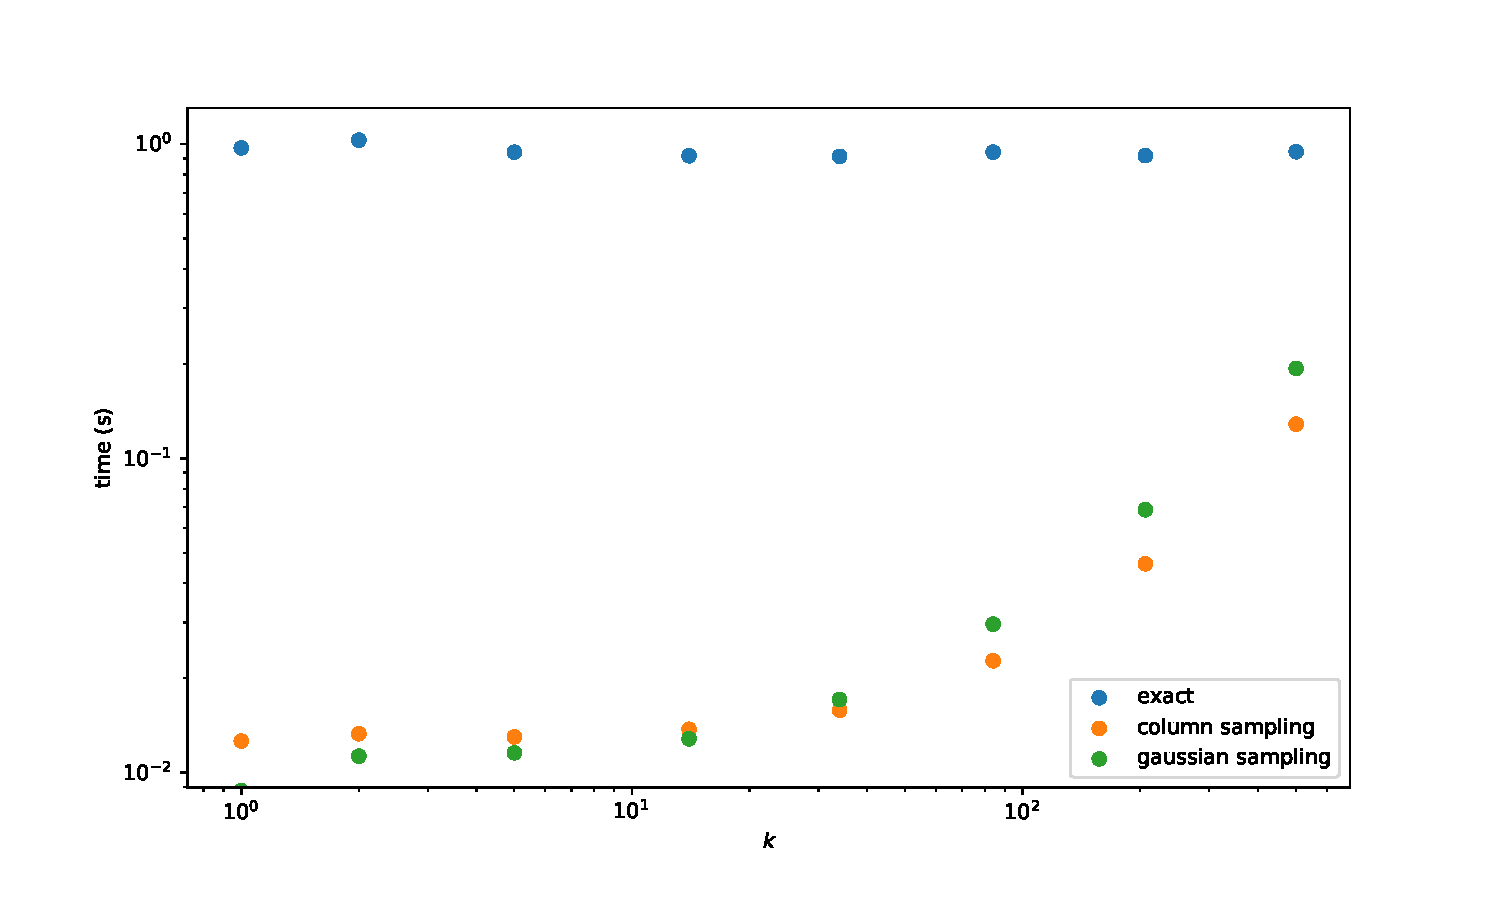
\includegraphics[width=\textwidth]{img/times.pdf}
            \caption{Runtime vs. rank of approximation}
            \label{runtimes}
        \end{figure}
        
        
        We also take \( s=k \), since there is no point computing the approximate SVD and then discarding extra information. Note further than since we are just looking to approximate the range we could use a QR factorization which would be faster than SVD (by a constant factor).

        The time to compute the approximations are shown in Figure~\ref{runtimes}. Note that the time to compute the optimal rank \( k \) approximation is independent of \( k \) since the full SVD must be computed. 
        

        Sample outputs are shown in Figures~\ref{opt},\ref{col},\ref{gaus}. Note that the images shown here have been downsampled to reduce the size of this document. 
    \begin{figure}[ht]\centering
            \foreach \i in {1,2,5,14,34,84,206,501}{
                \begin{subfigure}{.23\textwidth}
                    \includegraphics[width=\textwidth]{img/\i.png}
                    \caption{\( k=\i \)}
                \end{subfigure} 
            }
            \caption{optimal rank-\(k\) approximation via SVD truncation}
            \label{opt}
        \end{figure}
        
        \begin{figure}[ht]\centering
            \foreach \i in {1,2,5,14,34,84,206,501}{
                \begin{subfigure}{.23\textwidth}
                    \includegraphics[width=\textwidth]{img/\i_fast.png}
                    \caption{\( k=\i \)}
                \end{subfigure} 
            }
            \caption{rank-\(k\) approximation via column sampling}
            \label{col}
        \end{figure}

        \begin{figure}[ht]\centering
            \foreach \i in {1,2,5,14,34,84,206,501}{
                \begin{subfigure}{.23\textwidth}
                    \includegraphics[width=\textwidth]{img/\i_faster.png}
                    \caption{\( k=\i \)}
                \end{subfigure} 
            }
            \caption{rank-\(k\) approximation via Gaussian test matrix}
            \label{gaus}
        \end{figure}

       


\end{enumerate}


\end{solution}


\end{document}
